\chapter{Methods}\label{chap:methods}

\section{Technologies}
The SafeScript project utilizes a comprehensive stack of technologies to deliver a robust and efficient solution for identifying and addressing security vulnerabilities in software projects. 
The key technologies employed in this project include:

\begin{itemize}
\item \textbf{Django Framework}: A high-level Python web framework that encourages rapid development and clean, pragmatic design.
\item \textbf{Python}: The primary programming language used for developing the backend logic and machine learning models.
\item \textbf{SQLite v3}: A lightweight, disk-based database used for storing user credentials, project details, and scanning results.
\item \textbf{JavaScript}: Used for adding interactive elements to the web pages and handling client-side logic.
\item \textbf{HTML}: The standard markup language for creating web pages.
\item \textbf{CSS}: A style sheet language used for describing the presentation of the web pages.
\item \textbf{Bootstrap}: A front-end framework used for developing responsive and mobile-first web pages.
\item \textbf{Ajax}: A set of web development techniques used to create asynchronous web applications.
\item \textbf{jQuery}: A fast, small, and feature-rich JavaScript library used to simplify HTML DOM tree traversal and manipulation.
\item \textbf{GitPython}: A Python library used to interact with Git repositories.
\end{itemize}

\section{Implementation}
The implementation of the SafeScript project involves several key components and workflows designed to ensure seamless operation and effective vulnerability detection.

\subsection{User Options}
Users are provided with two primary options for submitting their code for analysis:
\begin{enumerate}
\item{\textbf{Single File Import}} Users can upload a single Python source file.
\item{\textbf{Repository Cloning}} Users can provide a link to a code repository (e.g., GitHub, Bitbucket), which the system will clone and analyze.
\end{enumerate}
\subsection{Core Functionalities}
The core functionalities of the system as follows:

\begin{enumerate}

\item{\textbf{User Authentication}}: Users authenticate themselves using a username and password to access the system.
\item{\textbf{Project Creation and Management}}: Users create and manage projects, selecting either to import a single file or clone an entire repository.
\item{\textbf{Code Retrieval}}: The system fetches the code from the specified source.
\item{\textbf{Model Selection}} During the vulnerability detection phase, users can choose between the ChatGPT API and the LSTM model. 
This flexibility allows users to leverage the strengths of both models, ensuring robust and reliable security analysis.
\item{\textbf{Data Conversion}}: The retrieved code is converted into word2vec (w2v) format, preparing it for vulnerability analysis.
\item{\textbf{Vulnerability Detection}}: Users can select either the integrated ChatGPT API or the LSTM model for vulnerability detection.
\item{\textbf{Report Generation}}: The system generates detailed reports outlining detected vulnerabilities, their severity, and recommendations for fixes.
\item{\textbf{Rescan Capability}}: Users can rescan their code after making fixes to ensure that vulnerabilities have been addressed.

\end{enumerate}

\subsection{Frontend and Backend Integration}
The frontend, built with HTML, CSS, Bootstrap, and JavaScript (including jQuery and Ajax), provides a user-friendly interface for interaction. 
The backend, developed using Django, handles the business logic, user authentication, project management, code retrieval, data conversion, vulnerability detection, and report generation. 
SQLite v3 is used for database management, ensuring efficient data storage and retrieval.

\subsection{AI Integration}
The AI integration in the SafeScript project leverages advanced machine learning models to enhance the accuracy and efficiency of vulnerability detection. 
At the moment the system is integrated with GPT API and LSTM model, which we have trained over past labs. 
Beside, those two the system have the capability to be integrated with other AI models as well.

\subsubsection{Integrated ChatGPT API}
The system integrates the ChatGPT API, enabling it to utilize the powerful capabilities of the ChatGPT model for analyzing code and identifying potential security vulnerabilities. 
This integration allows the system to provide context-aware analysis and generate comprehensive vulnerability reports.
This integration allows the user to detect deffirent types of vulnerabilities in their python code.

\subsubsection{LSTM Model}
In addition to the ChatGPT API, the system incorporates an in-house developed LSTM (Long Short-Term Memory) model. 
This model is specifically trained to detect security vulnerabilities in Python code. 
Users have the option to select the LSTM model for vulnerability detection, benefiting from its specialized focus and accuracy.
The LSTM model for has the capability to detect for specific type of vulnerabilities. The system can detect Cross-Site Scripting (XSS), Path Disclosure, Remote Code Execution, Command Injection.
The system has the capability to support more vulnerabilities types through LSTM model in the future.

By integrating these AI technologies, the SafeScript project enhances its capability to detect and report vulnerabilities effectively, providing users with actionable insights to improve the security of their software projects.

\section{Data Storage} 

The database for the Vulnerability Scanner project is structured using SQLite v3, providing a lightweight, disk-based database engine. This database includes several tables designed to handle user authentication, project management, and feedback functionalities.

The auth\_group table manages the different user groups within the system, facilitating role-based access control. The auth\_user table stores user information, including login credentials and profile details, to support user authentication and management. The auth\_user\_groups table links users to the groups they belong to, enabling group-based permissions and access control. Similarly, the auth\_user\_user\_permissions table maps individual users to specific permissions, allowing for fine-grained access control. The auth\_permission table defines various permissions that can be assigned to users or groups, ensuring secure and controlled access to different system functionalities.

The django\_admin\_log table records administrative actions performed within the system, providing an audit trail for monitoring and security purposes. The django\_content\_type table is used by the Django framework to keep track of all the models installed in the project, facilitating content type management. The authtoken\_token table stores authentication tokens for users, supporting secure API access.

For project-specific data, the main\_feedback table collects user feedback, including the subject and body of feedback messages, along with timestamps and user associations. The main\_price table manages pricing information related to the system's services or products, along with timestamps for creation and updates. The main\_response table records responses generated by the system, including response type, token usage, timestamps, and associated user and request information. The main\_log table logs user interactions with the system, capturing details such as user identity, URL accessed, user agent, IP address, request method, status code, and timestamps. Lastly, the main\_project table manages project information, including project identifiers, names, descriptions, repository details, status, timestamps, and associated user information.

These tables collectively support the core functionalities of the Vulnerability Scanner project, including user authentication, project management, feedback collection, and logging of interactions and administrative actions. This structured approach ensures efficient data management and retrieval, facilitating seamless operation and robust security.
% The database for the Vulnerability Scanner project is structured using SQLite v3, which provides a lightweight, disk-based database engine. This database includes several tables designed to handle user authentication, project management, and feedback functionalities. Below is a brief overview of the key tables:

% auth\\_group: This table manages the different user groups within the system, facilitating role-based access control.

% auth\\_user: This table stores user information, including login credentials and profile details, to support user authentication and management.

% auth\\_user\\_groups: This table links users to the groups they belong to, enabling group-based permissions and access control.

% auth\\_user\\_user\\_permissions: This table maps individual users to specific permissions, allowing for fine-grained access control.

% auth\\_permission: This table defines various permissions that can be assigned to users or groups, ensuring secure and controlled access to different system functionalities.

% django\\_admin\\_log: This table records administrative actions performed within the system, providing an audit trail for monitoring and security purposes.

% django\\_content\\_type: This table is used by the Django framework to keep track of all the models installed in the project, facilitating content type management.

% authtoken\\_token: This table stores authentication tokens for users, supporting secure API access.

% main\\_feedback: This table collects user feedback, including the subject and body of feedback messages, along with timestamps and user associations.

% main\\_price: This table manages pricing information related to the system's services or products, along with timestamps for creation and updates.

% main\\_response: This table records responses generated by the system, including response type, token usage, timestamps, and associated user and request information.

% main\\_log: This table logs user interactions with the system, capturing details such as user identity, URL accessed, user agent, IP address, request method, status code, and timestamps.

% main\\_project: This table manages project information, including project identifiers, names, descriptions, repository details, status, timestamps, and associated user information.

% These tables collectively support the core functionalities of the Vulnerability Scanner project, including user authentication, project management, feedback collection, and logging of interactions and administrative actions. This structured approach ensures efficient data management and retrieval, facilitating seamless operation and robust security.
Figure \ref{fig:dataStorage} shows the data storage in Sqlite database.

\begin{figure}[H]
    \centering
    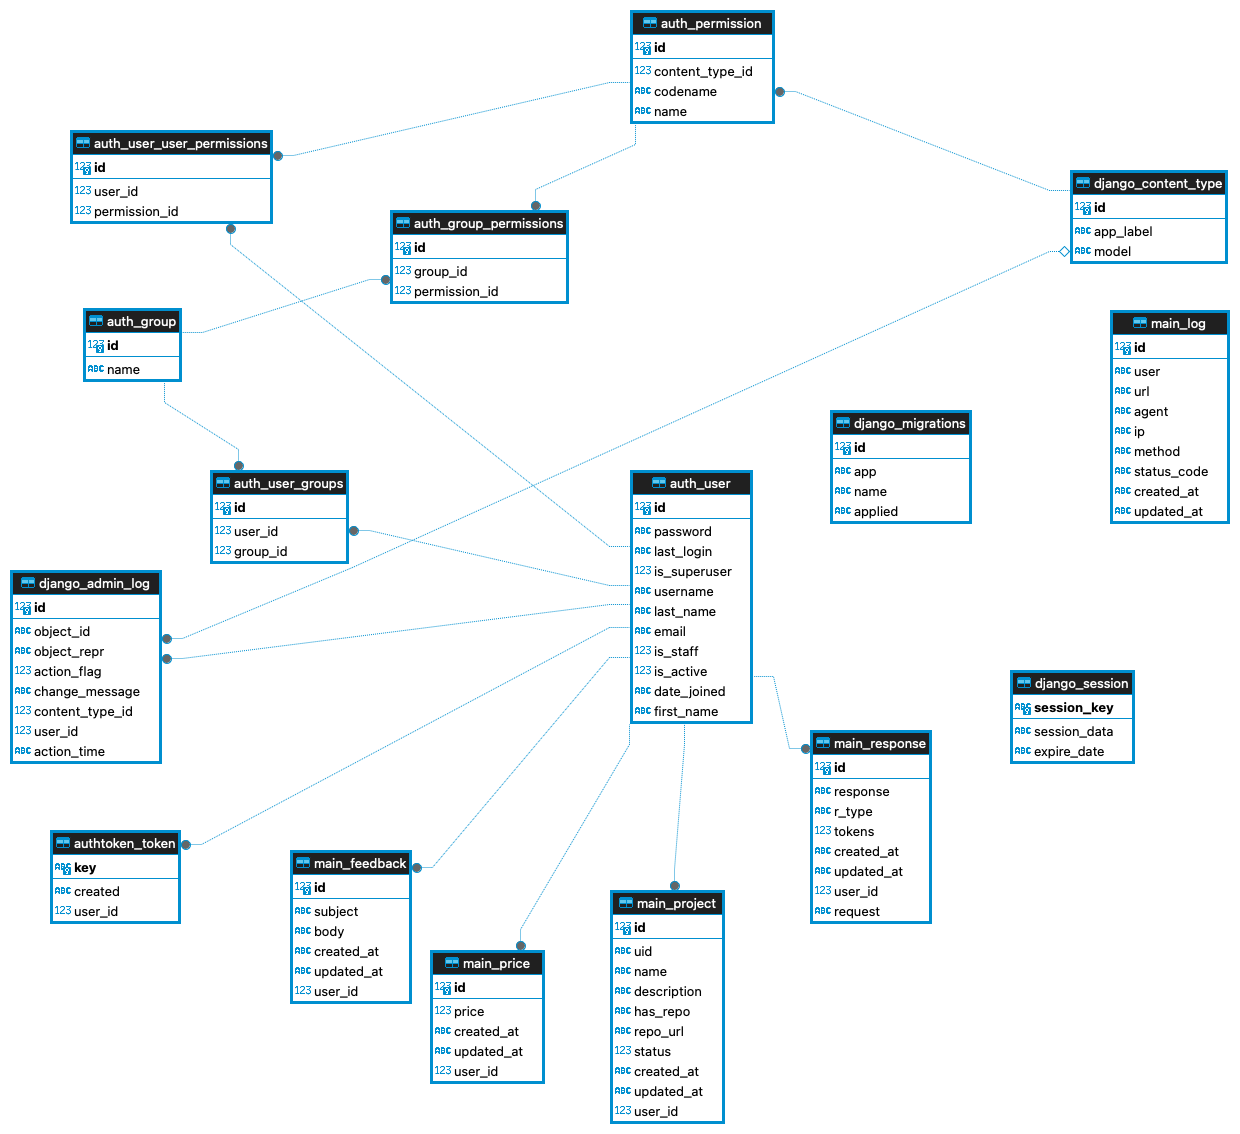
\includegraphics[width=0.9\linewidth]{images/ERD.png}
    \caption{System storage ER diagram}
    \label{fig:dataStorage}
\end{figure}

\section{Challenges}
The development and implementation of the Vulnerability Scanner project presented several challenges, particularly in the integration of AI models and prompt engineering. These challenges required innovative solutions to ensure seamless functionality and reliable performance.

\subsection{Integration of AI Models}
The integration of AI models posed a significant challenge due to the need to support both the ChatGPT API and our in-house LSTM model. Each model has distinct requirements and operational characteristics, necessitating careful planning and execution to ensure smooth integration.

\textbf{Challenge Details}:

\begin{enumerate}
\item \textbf{Different Architectures}: The ChatGPT API and the LSTM model operate on fundamentally different architectures. The ChatGPT API, provided by OpenAI, is a transformer-based model optimized for natural language understanding and generation, while the LSTM model is a recurrent neural network (RNN) variant designed specifically for sequential data analysis.
\item \textbf{API Integration}: Integrating the external ChatGPT API involved ensuring secure and efficient communication with the OpenAI servers, handling API requests and responses, and managing API rate limits and potential latency.
\item \textbf{Internal Model Management}: The LSTM model, being developed and hosted internally, required robust deployment infrastructure, including model serving, scaling, and maintenance.
\end{enumerate}

\textbf{Solution}:
\begin{enumerate}
    \item \textbf{Unified Interface}: We developed a unified interface that abstracts the differences between the two models. This interface allows the system to interact with either model seamlessly, providing a consistent experience regardless of the selected AI model.
    \item \textbf{API Wrapper}: For the ChatGPT API, we implemented a wrapper that handles API calls, error management, and response parsing. This wrapper ensures reliable communication and error handling when interacting with the external API.
    \item \textbf{Model Server}: For the LSTM model, we set up a dedicated model server using Django and REST framework, enabling efficient model inference requests and scalable deployment. 
    This server handles requests from the main application, processes the input data, and returns the analysis results.
    \item \textbf{Configuration Management}: A configuration management system was implemented to manage model-specific settings and parameters, allowing the system to dynamically switch between the ChatGPT API and the LSTM model based on user preference.
\end{enumerate}

\subsection{Prompt Engineering}
Prompt engineering was another critical challenge due to the variability in responses from the AI models. Effective prompt engineering is essential for obtaining accurate and relevant results from the models.

\textbf{Challenge Details}:
\begin{enumerate}
\item \textbf{Response Variability}: The ChatGPT model, in particular, can generate diverse responses depending on the prompt's phrasing. 
This variability can lead to inconsistent results, making it challenging to ensure the reliability of vulnerability detection.
\item \textbf{Context Management}: Ensuring that the models receive sufficient context to accurately analyze code and identify vulnerabilities required careful crafting of prompts.
\item \textbf{Error Handling}: Handling ambiguous or incorrect responses from the models necessitated robust error detection and correction mechanisms.
\end{enumerate}

\textbf{Solution}:

\begin{enumerate}
\item \textbf{Iterative Prompt Development}: We adopted an iterative approach to prompt development, continually refining the prompts based on testing and feedback. 
This iterative process involved experimenting with different prompt structures and evaluating their impact on response quality.
\item \textbf{Template-Based Prompts}: We designed template-based prompts that ensure consistency in the input provided to the models. These templates include placeholders for code snippets and context information, standardizing the prompts and reducing response variability.
\item \textbf{Context Enrichment}: To provide sufficient context, we implemented mechanisms to extract relevant information from the code and include it in the prompts. This includes details about the code structure, dependencies, and known issues.
\item \textbf{Post-Processing}: We developed post-processing algorithms to analyze and validate the responses from the AI models. These algorithms check for consistency, filter out irrelevant information, and ensure that the final output meets the required standards.
\end{enumerate}

By addressing these challenges through thoughtful solutions, we were able to integrate the AI models effectively and enhance the reliability of the Vulnerability Scanner project. 
This ensures that users receive accurate and actionable insights for improving the security of their software projects.
